\documentclass[11pt,twoside,a4paper]{article}
\usepackage[utf8]{inputenc}
\usepackage[english,german]{babel}
\usepackage{utopia}
\usepackage[margin=1in]{geometry}
\usepackage[parfill]{parskip}
\usepackage{makeidx}
\usepackage[onehalfspacing]{setspace}
\usepackage{graphicx}
\usepackage{fancyhdr}
\usepackage{lastpage}
\usepackage{hyperref}
\usepackage{multicol}
\renewcommand{\sffamily}{phv}

\newcommand{\titleText}{Spick Physikprüfung}
\newcommand{\authorText}{Janes Thomas, Patrick Günthard}
\newcommand{\dateText}{\today}

\title{\titleText}
\author{\authorText}
\date{\dateText}

\pagestyle{fancy}
\fancyhf{}

\fancyhead[EL]{\titleText}
\fancyhead[OR]{\authorText}
\cfoot{\thepage \space von \pageref{LastPage}}

\begin{document}
	\maketitle
	
	\section{Formeln}
	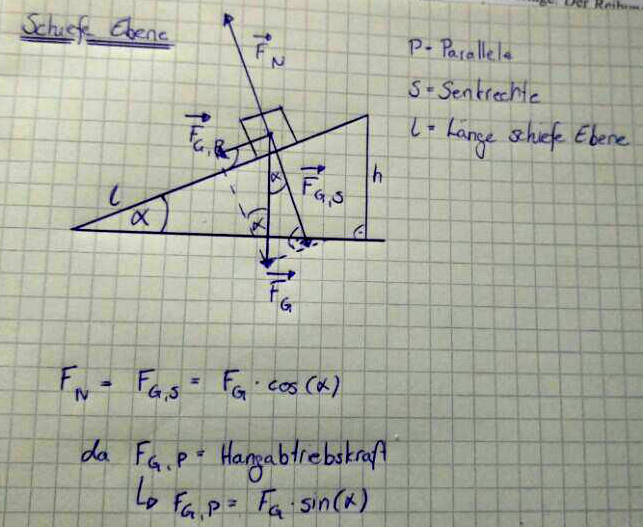
\includegraphics[width=8cm]{se1a}
	
	\begin{multicols}{2}
		\subsection{Kraft (allgemein)}
		\(F = m * a\)
		\subsection{Hangantriebskraft}
		\(F_{G,P} = F_G * sin(\alpha)\)
		\subsection{Normalkraft}
		\(F_{G,S} = F_N = \cos\alpha*F_G\)
		\subsection{Reibungskraft}
		\(F_R = F_N * \mu\)
		\subsection{Kräftezerlegung auf der schiefen Ebene}
		\subsection{Gekoppelte Körper}
		\subsection{Steigung \% - Grad}
		\(\alpha = \arctan(m) \)
	\end{multicols}
	
	\section{Beispiele}
	
	\subsection{Heruntergleitender Körper aufhalten, mit Reibung}
	
	\(F_X = F_{G,P} - F_R \)
	
\end{document}